\documentclass[12pt]{article}

\baselineskip=20pt
\hsize=340pt
\vsize=490pt

\usepackage{amssymb}

\usepackage{color,graphicx}

\usepackage{amsmath}


\usepackage{amsmath,amssymb,amsthm}
\usepackage{pb-diagram}
%%%%%%%%%%%%%%%%%%%%%%%%%%%%%%%%%%%%%%%%%%%%%%%%%%%%%%%%%%%%%%%%%%%%%%%%%%%%%%%%%%%%%%%%%%%%%%%%%%% 
\usepackage{multicol}
\usepackage{color}
\usepackage{hyperref}
\usepackage{graphicx}
\usepackage[utf8x]{inputenc}
\usepackage[english]{babel}

\newtheorem{Def}{Definition}[section]
\newtheorem{theorem}{Theorem}
\newtheorem{statement}{Statement}
\newtheorem{Cnj}[Def]{Conjecture}
\newtheorem{Prop}[Def]{Property}
\newtheorem{example}{Example}[section]


\newcommand{\go}{\stackrel{\circ }{\mathfrak{g}}}
\newcommand{\ao}{\stackrel{\circ }{\mathfrak{a}}}
\newcommand{\co}[1]{\stackrel{\circ }{#1}}
\newcommand{\pia}{\pi_{\mathfrak{a}}}
\newcommand{\piab}{\pi_{\mathfrak{a}_{\bot}}}
\newcommand{\gf}{\mathfrak{g}}
\newcommand{\gfh}{\hat{\mathfrak{g}}}
\newcommand{\af}{\mathfrak{a}}
\newcommand{\afh}{\hat{\mathfrak{a}}}
\newcommand{\bff}{\mathfrak{b}}
\newcommand{\afb}{\mathfrak{a}_{\bot}}
\newcommand{\hf}{\mathfrak{h}}
\newcommand{\hfg}{\hf_{\gf}}
\newcommand{\hfa}{\hf_{\af}}
\newcommand{\hfb}{\mathfrak{h}_{\bot}}
\newcommand{\pf}{\mathfrak{p}}
\newcommand{\aft}{\widetilde{\mathfrak{a}}}
\newcommand{\sfr}{\mathfrak{s}}


\begin{document}

\title{Splints of root systems for special Lie subalgebras}

\author{V.D.~Lyakhovsky$^1$, A.A.~Nazarov$^{1,2}$, P.I.~Kakin$^{1}$\\
  {\small $^1$ Department of High-energy and elementary particle physics,}\\ {\small St Petersburg State University}\\
  {\small 198904, Saint-Petersburg, Russia,}\\
  {\small $^{2}$ e-mail: antonnaz@gmail.com}}
%\date{}
%\address{ $^1$ Department of High-energy and elementary particle physics,  St Petersburg State University, 198904, Saint-Petersburg, Russia}
%\address{ $^{2}$ e-mail: anton.nazarov@hep.phys.spbu.ru}

\maketitle

\begin{abstract}
  Splint is a decomposition of root system into a union of root systems. Splint of root system for a
  simple Lie algebra appears naturally in the studies of (regular) embeddings of reductive
  subalgebras. Splint can be used to construct branching rules. We consider a special embedding of a
  Lie subalgebra into a simple Lie algebra. We classify the projections of algebra root systems and
  single out the conditions of splint appearance and coincidence of branching coefficients with
  weight multiplicities. While such a coincidence is not very common it is connected with
  Gelfand-Tsetlin basis.

\noindent{\it Keywords\/}: Lie algebra, special subalgebra, branching, weight multiplicity, splint
\end{abstract}


\section{Introduction}
\label{sec:introduction}

The notion of splint was introduced by David Richter in the paper \cite{richter2008splints}. Splint
is a decomposition of a root system into a disjoint union of the images of two or more embeddings of some
other root systems. An embedding $\phi$ of a root system $\Delta_1$ into a root system $\Delta$ is a
bijective map of roots of $\Delta_{1}$ to a (proper) subset of $\Delta$ that commutes with the vector
composition law in $\Delta_{1}$ and $\Delta$.
\begin{equation*}
\phi:\Delta_1 \longrightarrow \Delta
\end{equation*}
\begin{equation*}
\phi \circ (\alpha + \beta) =\phi \circ \alpha + \phi \circ \beta,
\,\,\, \alpha,\beta \in \Delta_1
\end{equation*}

Note that the image $Im(\phi)$ is not required to inherit the root system properties except the
addition rules equivalent to the addition rules in $\Delta_{1}$ (for pre-images). If an embedding
$\phi$ preserves the angles between the roots it is called ``metric''. Two embeddings $\phi_1$ and
$\phi_2$ can splinter $\Delta$ when the latter can be presented as a disjoint union of images
$Im(\phi_1)$ and $Im(\phi_2)$.

Why one would consider non angle-preserving maps of root systems? Additive properties of the root system
determine the structure of the Verma module:
    \begin{equation*}
      M^{\mu}=U(\gf)\underset{U(\bff_{+})}{\otimes} D^{\mu}(\bff_{+})=\{(E^{-\alpha_{1}})^{n_{1}}\dots (E^{-\alpha_{s}})^{n_{s}} \left|v_{\mu}\right>\}_{\alpha_{i}\in\Delta^{+}}^{n_{i}=0,1,\dots}
    \end{equation*}
Here $\bff_{+}$ is the Borel subalgebra of $\gf$, $D^{\mu}$ is its one-dimensional representation,
$\left|v_{\mu}\right>$ is the highest weight vector and $E^{-\alpha_{j}}$ are lowering operators
that are in correspondence with positive roots $\alpha_{j}\in \Delta^{+}$. 
The Weyl character formula expresses a character of an irreducible representation as a combination of
the characters of the Verma modules: 
\begin{equation*}
  \mathrm{ch} L^{\mu}=\frac{\sum_{w\in W} \varepsilon(w) e^{w(\mu+\rho)-\rho}}{\sum_{w\in W}\varepsilon(w) e^{w\rho-\rho}}=\sum_{w\in W} \varepsilon(w)\; \mathrm{ch} M^{w(\mu+\rho)-\rho}
\end{equation*}
Here the sum is over elements of the Weyl group and their actions $w\triangleright \mu
=w(\mu+\rho)-\rho$ depend on angles between roots. But we can rewrite the Weyl character formula
representing the Weyl group elements as the products of the reflections $s_{\alpha}, \alpha \in S$ in
the hyperplanes orthogonal to the simple roots: $w=s_{\alpha_{1}}\cdot s_{\alpha_{2}}\dots$. The reflections act
on the root system by permutations, so the composition of such an action with the embedding $\phi$ is easily
obtained. The orbit of the Weyl group action $w\triangleright \mu, w\in W$, can be constructed by
subtractions of roots from the highest weight $\mu$. Let's denote the Dynkin labels of $\mu$ by
$(\mu_{1},\dots \mu_{r})$. Then $\mu-\mu_{1}\alpha_{1}, \mu-\mu_{2}\alpha_{2},\dots,
\mu-\mu_{r}\alpha_{r}, \alpha_{i}\in S$, are the points of the orbit that can be obtained by
the elementary reflections $s_{\alpha_{i}}, \alpha_{i}\in S$. The next set of points that are obtained by
two consecutive reflections $s_{\alpha_{i}}\cdot s_{\alpha_{j}}\triangleright\mu$ are obtained as
the subtraction $\mu-\mu_{i}\alpha_{i}-\mu_{j} (s_{\alpha_{i}}\alpha_{j})$. Continuing this way we
construct the image of the singular element $\Psi=\sum_{w\in W} \varepsilon(w) e^{w(\mu+\rho)-\rho}$
after the embedding $\phi$ \cite{2011arXiv1111.6787L}. The multiplicities in the character of the Verma
module are unchanged by the embedding since they are determined by the additive properties of the roots.
So we see that the weight multiplicities of irreducible modules are also preserved by the embedding.

The root system of the regular subalgebra is contained in the root system of the algebra so the splint is useful in the
computation of branching coefficients. 

In the paper \cite{2011arXiv1111.6787L} it was proven that the existence of splint leads to the
coincidence of branching coefficients with weight multiplicities under certain conditions. We denote a
Lie algebra by $\gf$ and consider it's subalgebra $\af$. If $\af$ is a regular subalgebra, its root
system $\Delta_{\af}$ is contained in $\Delta_{\gf}$. Branching coefficients $b^{(\mu)}_{\nu}$
appear in the decomposition of an irreducible representation $L^{\mu}_{\gf}$ of $\gf$ to the sum of
irreducible representations of $\af$:
\begin{equation}
  \label{eq:1}
  L^{\mu}_{\gf}=\bigoplus_{\nu} b^{(\mu)}_{\nu} L^{\nu}_{\af}
\end{equation}

Assume that the root system $\Delta_{\gf}$ splinters as $\Delta_{\gf}=\Delta_{\af} \cup
\phi(\Delta_{\sfr})$, where $\phi$ is an embedding of a root system $\Delta_{\sfr}$ of some semisimple
Lie algebra $\sfr$. Then branching coefficients $b^{(\mu)}_{\nu}$ for the reduction
$L^{(\mu)}_{\gf\downarrow \af}$ coincide with the weight multiplicities $m^{(\tilde \mu)}_{\nu}$ in the $\sfr$-representations provided certain technical condition holds \cite{2011arXiv1111.6787L}.
The highest weight $\tilde\mu$ of the $\sfr$-representation is calculated from the Dynkin labels of the highest
weight $\mu$ of the $\gf$-module.
The proof of the coincidence of the branching coefficients with the weight multiplicities of
$\sfr$-module is based upon the decomposition of singular element of the algebra $\gf$ into singular
elements for $\sfr$:
\begin{equation}
 \Phi ^{\mu }_{\gf} = \sum_{w\in W_{\frak{a}}}\epsilon\left( w\right)w\left( e^{\mu +\rho _{\gf}}\phi\left( e^{-\widetilde{\mu }}\Psi^{\widetilde{\mu }}_{\sfr}\right)\right),
\end{equation}
where $\epsilon\left( w\right)$ is a determinant of the element $w$ of the Weyl group $W_{\af}$ of
the subalgebra $\af$. The action of the Weyl group on the weights is extended to the algebra of formal
exponents by the rule $w\left(e^{\nu}\right)=e^{w\nu}, w\in W$. Hence, the multiplicity $M_{\left(
      \sfr\right) \widetilde{\nu }}^{\widetilde{\mu }}$ of the weight $\widetilde{\nu }$ from the
  weight diagram of the algebra $\sfr$ with the highest weight $\tilde\mu$ defines the branching
  coefficient $b_{\nu }^{(\mu )}$ for the highest weight $\nu =\left( \mu -\phi \left(
      \widetilde{\mu }-\widetilde{\nu }\right) \right) $:
\begin{equation}
b_{\left( \mu -\phi \left( \widetilde{\mu }-\widetilde{\nu }\right) \right)
}^{(\mu )}=M_{\left( \sfr\right) \widetilde{\nu }}^{\widetilde{\mu }}. 
\label{bran1}
\end{equation}

We use similar approach to study special embeddings. We consider special embeddings of Lie
subalgebras into a Lie algebra. In this case the root system of the subalgebra is not contained in
the root system of the algebra. So the original motivation for splints is not applicable. But we can
consider the projection of the root system of the algebra on the root space of the subalgebra. Such
a projection is not a root system anymore, but it satisfies milder conditions (Section
\ref{sec:spec-embedd-proj}). It is possible to classify the splints of the projection using the fact
that the adjoint representation of the algebra is decomposed into the direct sum of representations
of the subalgebra. We show that if there is a splint then branching coefficients coincide with
weight multiplicities of representations of another Lie algebra (Section
\ref{sec:splints-spec-embedd}). Thus in this case branching coefficients are very easy to compute.

The use of representation theory of the subalgebra allows us to classify all the splints for the projections
of the algebra root system. We also apply this method to metric splints and regular subalgebras and get
a unified treatment. We obtain the Gelfand-Tsetlin rules for regular and special embeddings this way.

In conclusion \ref{sec:conclusion} we discuss the cases when the projection of the root system does
not fall into the classification mentioned above.


\section{Special embeddings and projections of root system}
\label{sec:spec-embedd-proj}

The study of specialy embedded subalgebras traces back to the fundamental papers by Eugene Dynkin
\cite{dynkin1952semisimple,dynkin1952maximal} where he called such subalgebras ``S-subalgebras'' to
distinguish from regular or ``R-subalgebras'' that have root systems obtained by dropping some roots
of the algebra root system. Thus regular subalgebras are easy to construct by dropping nodes from
the extended Dynkin diagram of the algebra, while the case of special subalgebras is more difficult. The complete
classification for exceptional Lie algebras was obtained recently in \cite{minchenko2006semisimple}.
The algorithm of the special subalgebras construction is available in GAP package but still requires
a manual intervention \cite{de2011constructing}.  

Assume that the Lie algebra $\gf$ is simple. Let's denote a subalgebra by
$\af$. We denote corresponding Cartan subalgebras by $\hfg$ and $\hfa$ and identify them with the dual
spaces $\hfg^{*}$, $\hfa^{*}$ using the Killing forms of $\gf$ and $\af$.

To construct an embedding $\af\to\gf$ consider some representation $L^{\nu}_{\af}$ as a subspace of
Lie algebra $\gf$. Then one needs to check that the generators of $\af$ can be presented as
linear combinations of generators of $\gf$. We can identify the Cartan subalgebra $\hfa\subset \af$ with
the dual space $\hfa^{*}$ using the Killing form. Then the root system $\Delta_{\gf}$ of $\gf$ can be
projected to $\hfa^{*}$ using the expression of $\hfa$-generators through $\hfg$-generators.

%%  To reduce $\gf$-representations project $\gf$ root system to Cartan subalgebra of $\af$. 
%% 
%%  To construct an embedding of special subalgebra $\af\to \gf$ one
%% needs to consider some representation of $\af$ of dimension $\mathrm{dim}\gf$ and
%% identify generators of $\af$ with linear combinations of generators of $\gf$ in
%% the adjoint representation. 
%% 
%%  Such subalgebras are constructed by considering
%% representation of the algebra to
%% 

This projection is described in the classical papers \cite{dynkin1952semisimple,dynkin1952maximal} by the following theorem:

\begin{theorem}\label{dyn0}
  If a representation $L^{\mu}_{\gf}$ of the algebra $\gf$ induces a representation
  $L^{\tilde\mu}_{\af}$ on the subalgebra $\af$ then the weight system of $L^{\tilde\mu}_{\af}$ can
  be obtained from $L^{\mu}_{\gf}$ by an orthogonal projection of $\hfg^{*}$ on $\hfa^{*}$.

  \cite{dynkin1952maximal}. 
\end{theorem} 

In relation to the adjoint representation of $\gf$ this theorem means that the projection of the root system $\Delta_{\gf}$ to $\hfa^{*}$ is a weight system of some
finite-dimensional but not irreducible representation of $\af$. Moreover this reducible representation contains the adjoint representation of $\af$. And if we denote such a projection by
\begin{equation}
  \label{eq:2}
  \Delta'=\pia\left(\Delta_{\gf}\right),
\end{equation}
then the roots of $\af$ will be contained in $\Delta'$. Thus the system $\Delta'$ can be a root
system but it might not be reduced and might contain some vectors with multiplicities greater than
one.

The following theorems \cite{dynkin1952semisimple} also concern the properties of $\Delta'$. 

\begin{theorem}\label{dyn1}
  Every special subalgebra $\af$ of a semisimple Lie algebra $\gf$ is integer, i.e. the projections of
  the roots of $\gf$ to $\hfa^{*}$ are linear combinations of the simple roots of $\af$ with integer
  coefficients \cite{dynkin1952semisimple}
\end{theorem}

\begin{theorem}\label{dyn2}
  If $\af$  is a semisimple subalgebra of a semisimple Lie algebra $\gf$ and the generator $e_{\alpha}$ corresponding to
  the root $\alpha$ of $\af$ is presented as a linear combination $e_{\alpha}=\sum_{\beta}
  e_{\beta}$ of $\gf$-generators
  corresponding to the roots $\beta$ of $\gf$, then the roots $\beta$ are projected into $\alpha$,
  $\pia(\beta)=\alpha$. 
  \cite{dynkin1972semisimple,dynkin1952semisimple}. 
\end{theorem}

From these theorems we see that the root system $\Delta_{\af}$ is metrically embedded (in the sense
of splint) into the projection $\Delta'$. Moreover, the multiplicities of some roots
$\alpha\in\Delta_{\af}$ in this projection $\Delta'$ are greater than one. 

For example the projection of the root system of $D_{4}$($so(8)$) to the root system of the special
subalgebra $A_{2}$($su(3)$) coincides with the root system $G_{2}$, but the short roots have the multiplicity $3$.


%% Relying on these theorems we can encode the projections of root system by Dynkin diagrams. We need
%% to allow simple roots to have non-trivial multiplicities. 
%% 

\section{Splints for special embeddings}
\label{sec:splints-spec-embedd}

%Since roots are weights of the adjoint representation, such a projection produces the weight diagram
%of $\af$-representation that contains adjoint representation of $\af$.
%After the subtraction of
%$\af$-root system $\Delta_{\af}$ from $\Delta'$ we obtain the weight diagram of representation called
%``characteristic representation of subalgebra $\af$'' by Dynkin in the seminal paper
%\cite{dynkin1952semisimple}.

We want to classify all the cases when branching coefficients coincide with weight multiplicities of
some other algebra representations. Such a coincidence is possible when the projection $\Delta'$ of
the $\gf$ root system admits a splint $\Delta'=\varphi_{\af}(\Delta_{\af})\cup
\varphi_{\sfr}(\Delta_{\sfr})$, where $\varphi_{\af}$ and $\varphi_{\sfr}$ are the embeddings of
the corresponding root systems. The embedding $\varphi_{\af}$ is metric and trivial. Moreover, the
projection of the singular element $\pia\left(\Psi^{\mu}_{\gf}\right)$ should admit a decomposition into
a linear combination of singular elements of irreducible representations of $\sfr$:
\begin{equation}
  \label{eq:4}
  \pia\left(\Psi^{\mu}_{\gf}\right)=\sum_{\nu} \varkappa_{\nu}e^{\nu}\Psi^{\tilde\mu}_{\sfr},
\end{equation}
with integer coefficients $\varkappa_{\nu}$, where the sum is over the set of weights $\nu$ that
will be determined later. Such a decomposition of the singular element is very similar to the branching of Weyl group orbits considered in the papers \cite{larouche2011branching,larouche2009branching}. First we classify all the splints of the projection of a root system into
a union of simple root systems for special embeddings, and then discuss the decomposition of singular
elements.

Projection of the $\gf$ root system $\Delta'$ coincides with the projection of the weight diagram of the
adjoint representation of the algebra $\gf$ with the exception of zero weight. The adjoint representation of
$\gf$ contains the adjoint representation of $\af$ and can be decomposed as
\begin{equation}
  \label{eq:3}
  \mathrm{ad}_{\gf}=\mathrm{ad}_{\af}\oplus M_{\af}^{\chi},
\end{equation}
where $M^{\chi}_{\af}$ is not necessary irreducible representation of $\af$ called
``characteristic'' in \cite{dynkin1952semisimple}. 

The weight diagram of $M^{\chi}_{\af}$ coincides with the root system $\Delta_{\sfr}$ with the exception of
zero weight. So we need to find all the representations for all simple Lie algebras $\af$, such that
their weight diagrams are root systems after the exclusion of zero weight. In order to do so we must
note, that all the weights of $M^{\chi}_{\af}$ should have a length not less than the length of the shortest
root of $\af$, since $\af$ is an integer subalgebra of $\gf$ \ref{dyn1}. Moreover, $M^{\chi}_{\af}$
should contain weights of at most two different lengths. 

If the root system $\Delta_{\gf}$ contains roots $\alpha: \alpha\perp \beta,\; \forall \beta\in
\Delta_{\af},$ orthogonal to the root system of the subalgebra, one cannot proceed with the decomposition
of the singular element \ref{eq:4}. The elements $e^{\nu}$ of $\pia\left(\Psi^{\mu}_{\gf}\right)$
should be augmented with the dimensions of representations of the algebra $\afb$ spanned by generators
corresponding to the orthogonal roots \cite{2010arXiv1007.0318L}. Then there will be non-trivial
multiplicities in the right hand side of \ref{eq:4} and no coincidence of branching coefficients
with the weight multiplicities of $\sfr$-representations. One can write more cumbersome relation between
the multiplicities and branching coefficients, but it is out of scope for the present paper.

The multiplicity of zero weight in the adjoint representation is equal to the rank of the algebra. So if
$\mathrm{rank}\gf-\mathrm{rank}\af=1$, the representation in question $M^{\chi}_{\af}$ must be
multiplicity-free. If $\mathrm{rank}\gf-\mathrm{rank}\af>1$ only zero weight can have non-trivial
multiplicities. 

The simplest class of multiplicity-free representations is called ``strongly multiplicity free''
\cite{lehrer2006strongly} and consists of multiplicity free representations with weight systems
admitting strict ordering $\nu_{1}<\nu_{2} \Leftrightarrow \nu_{1}=\nu_{2}+n \alpha$, where $n\in
\mathbb{N}, \alpha\in \Delta^{+}_{\af}$ and for all $\nu_{1},\nu_{2}$ either $\nu_{1}<\nu_{2}$ or
$\nu_{2}<\nu_{1}$.

The list of strongly multiplicity free representations consists of (first) fundamental representations
for the series $A_{r}, B_{r}, C_{r}$, the exceptional Lie algebra $G_{2}$ (7-dimensional representation) and
all $A_{1}$ representations. 

Fundamental weights of the algebra $A_{r}$ are shorter than its roots, but the projections of $\gf$
weights must be given by linear combinations of the roots of the  special subalgebra $\af$ with integer
coefficients, so the first class of strongly multiplicity free representations does not produce such a
projection. 

Nevertheless, the union of diagrams of the two fundamental representations of $A_{2}$ with the root
system of $A_{2}$ produces a weight diagram of $G_{2}$. This case corresponds to splint
$\Delta_{G_{2}}=\varphi_{1}( \Delta_{A_{2}})\cup \varphi_{2}(\Delta_{A_{2}})$ which is connected
with the regular subalgebra $A_{2}\subset G_{2}$ (see \cite{2011arXiv1111.6787L}).


The first fundamental representation of $B_{r}$ immediately gives us the splint $\Delta'=\pi_{B_{r}}\left(
\Delta_{D_{r+1}}\right) = \Delta_{B_{r}}\cup \Delta_{A_{1}+\dots+A_{1}}$ corresponding to the Gelfand-Tsetlin
multiplicity-free branching for the special embedding $\mathfrak{so}(2r+1)\to \mathfrak{so}(2r+2)$. 

The length of the first fundamental weight of  $C_{r}$ is less than the length of its short root, so
this case can not correspond to an integer subalgebra. 

If there are vectors of a different length in the projection $\Delta'$ on the subalgebra $A_{1}$, such a
projection is not multiplicity free, and $\Delta_{\sfr}$ contains parallel roots. The simplest case
is the special embedding $A_{1}\to A_{2}$ with index 4 where $\Delta_{\sfr}$ is the root system
$BC_{1}$. Such systems do not correspond to semisimple Lie algebras, so we can not speak of a
coincidence of branching coefficients for the reduction $\gf\downarrow \af$ with weight
multiplicities of $\sfr$-representations.

%% The only case of the projection $\Delta'$ to $A_{1}$ with root multiplicities not greater than 2 is
%% special embedding $A_{1}\to A_{2}$ with index 1 given by 
%% 
The weight diagram of the seven-dimensional representation of $G_{2}$ together with the $G_{2}$ root system
form the projection of the root system $B_{3}$ which corresponds to the special embedding 
$G_{2}\to B_{3}$. The branching coefficients in this case coincide with the weight multiplicities of
representations of algebra $\sfr=A_{2}$ with the image of the root system consisting of the short roots of
$G_{2}$. 

The complete classification of multiplicity-free irreducible representations was obtained in
\cite{howe1995perspectives} (see also \cite{stembridge2003multiplicity}). It consists of minuscule
and quasi-minuscule representations.

The weight $\mu$ is minuscule if $\left<\mu,\alpha^{\vee}\right>\leq 1$ for all $\alpha\in
\Delta^{+}$ and all the weights of the irreducible representation $L^{\mu}$ lie on the Weyl
group orbit of $\mu$. A weight is quasi-minuscule if $\left<\mu,\alpha^{\vee}\right>\leq 2$ for all
$\alpha\in \Delta^{+}$ and all non-zero weights lie on the single Weyl group orbit.

Minuscule representations are well-studied and very useful in the computations of e.g. tensor products
\cite{stembridge2003multiplicity,stembridge2001computational}. The minuscule representations are
indexed by the weight lattice modulo the root lattice. There is a unique quasi-minuscule
representation that is not minuscule for each simple Lie algebra. The multiplicity of the zero 
weight in quasi-minuscule representation is the number of the short nodes of the Dynkin diagram.

The list of the minuscule representations consists of tensor powers of the vector
representation for the series $A_{r}$; spin representations for the series
$B_{r}$; vector representations for $C_{r}$; vector and two half-spin for $D_{r}$; two
27-dimensional representations for $E_{6}$ and the 56-dimensional representation of $E_{7}$. 

Quasi-minuscule representations that are not minuscule are: the adjoint representation of $A_{r}$,
the vector representation for $B_{r}$, the $2r^{2}-r-1$-dimensional representation for $C_{r}$, the adjoint
representations for $D_{r}, E_{6}, E_{7}, E_{8}$, the 26-dimensional representation for $F_{4}$ and
the 7-dimensional of $G_{2}$.

%% 
%%     An (n+1
%%     k) for 0 ≤ k ≤ n (exterior powers of vector representation). Quasi-minuscule: n2+2n (adjoint)
%%     Bn 1 (trivial), 2n (spin). Quasi-minuscule: 2n+1 (vector)
%%     Cn 1 (trivial), 2n (vector). Quasi-minuscule: 2n2–n–1 if n>1
%%     Dn 1 (trivial), 2n (vector), 2n−1 (half spin), 2n−1 (half spin). Quasi-minuscule: 2n2–n (adjoint)
%%     E6 1 , 27, 27. Quasi-minuscule: 78 (adjoint)
%%     E7 1, 56. Quasi-minuscule: 133 (adjoint)
%%     E8 1. Quasi-minuscule: 248 (adjoint)
%%     F4 1. Quasi-minuscule: 26
%%     G2 1. Quasi-minuscule: 7
%% 
%% 

The classification of the multiplicity-free irreducible highest weight modules $L^{\mu}$ in
\cite{howe1995perspectives,stembridge2003multiplicity} consists of the following classes:
\begin{itemize}
\item (1) $\mu$ is minuscule,
\item (2) $\mu$ is quasi-minuscule and Lie algebra has only one short simple root,
\item (3) Lie algebra is $\mathfrak{sp}(6)$ and $\mu=\omega_{1}$, or
\item (4) Lie algebra is $\mathfrak{sl}(n + 1)$ and  $\mu= m\omega_{1}$ or $\mu  = m\omega_{n}$ 
\end{itemize}

We see that the case (1) contains strongly multiplicity free modules of the series $A_{r}$ and the exceptional
Lie algebra $G_{2}$, the class (2) contains strongly multiplicity free modules of $ B_{r}$ and $C_{r}$ ,
strongly multiplicity free modules of $A_{1}$ are included in the class (4).

We do not need to consider the minuscule representations for the simply-laced Lie algebras, since in this
case the length of the weights of the representation $M^{\chi}_{\af}$ is less than the length of the $\af$ roots,
that contradicts to $\af$ being an integer subalgebra. For the series $B_{r}$ we have already
discussed the minuscule spin representation, since it is strongly multiplicity free. The last case in
(1) is the vector representation for $C_{r}$. It is $2r$-dimensional, but the length of its highest weight $\omega_{1}$ is less
than the length of the short root of algebra $C_{r}$. So it can not be a characteristic representation
for the special subalgebra. 

%% , so with the dimension of the
%% adjoint representation we get $2r+2r^{2}=2r(r+1)$ which is exactly the dimension of the adjoint
%% representation for the algebra $D_{r+1}$.  
%% But there is no such embedding (?).
%% 
The case (2) consists of the series $B_{r}$ and the exceptional root system $G_{2}$. The embedding $G_{2}\to
B_{3}$ was already discussed. 
 The dimension of the adjoint representation for the series $B_{r}$
is $2r^{2}+r$ and of the quasi-minuscule representation it is $2r+1$, so the dimension of the algebra
$\gf$ should be $(r+1)(2r+1)$ with the $\mathrm{rank}\gf=r+1$. The only solution is $\gf=D_{r+1}$
and we have already seen that this case corresponds to the strongly multiplicity free module and
the Gelfand-Tsetlin basis.

In the case (3) the diagram of the representation contains weights with the length smaller than the
length of the short root, so it cannot be a projection of $\Delta_{\gf}$ to an integer subalgebra. 

We need to consider representations of the class (4) only for $m=1,2$ since the root system $\Delta_{\sfr}$
can have roots of at most two different lengths. In the case $m=1$ we get strongly multiplicity free
modules of $A_{r}$ which were discussed above. And for algebra $A_{2}$ and $m=2$ the weight diagram
of the representation $L^{2\omega_{1}}_{A_{2}}$ coincides with the root system of the exceptional Lie algebra
$G_{2}$. This case appears in the special embedding $A_{2}\to B_{3}$. But for $A_{r}, r>2$ there are
no root systems that coincide with the weight diagram of $L^{2\omega_{1}}_{A_{r}}$. 

So far we've considered all the cases when $\mathrm{rank}\gf-\mathrm{rank}\af=1$. To complete our
classification of splints we need the classification of all the representations where multiplicities
of all non-zero weights are equal to one. Fortunately, such a classification was obtained in
\cite{plotkin1998visual}. It consists of multiplicity-free representations and adjoint
representations of algebras $A_{r}, B_{r}, C_{r}$, $F_{4}$ and $G_{2}$. 

In order to have the embedding $\af\to \gf$ such that the adjoint representation of $\gf$ is
decomposed into two adjoint representations of $\af$ (and possibly several trivial
representations) we need to satisfy the following conditions:
\begin{itemize}
\item Denote by $n_{\gf}$ the total number of roots in $\Delta_{\gf}$ and the projection $\Delta'$.
  Then
  \begin{equation}
    \label{eq:5}
    n_{\gf}=2n_{\af}.
  \end{equation}
\item Denote rank of $\gf$ by shorthand notation $r_{\gf}$. Then the dimension
  \begin{equation}
    \label{eq:6}
    \mathrm{dim}\gf=n_{\gf}+r_{\gf}\geq 2\mathrm{dim}\af=2n_{\af}+2r_{\af}
  \end{equation}

\end{itemize}

% (? check with \cite{berenshtein1990multiplicity}).

For the adjoint representation of algebra $A_{r}$ we see that the projection $\Delta'$ of the root system
$\Delta_{\gf}$ should consist of roots of the subalgebra $\af=A_{r}$ with the multiplicity 2. The total
number of the roots for $A_{r}$ is $r(r+1)$, so $\Delta'$ and $\Delta_{\gf}$ contain $2r(r+1)$ roots,
since there are no roots orthogonal to $\Delta_{\af}$. There are two possible solutions for
$\gf$: $D_{r+1}$ and $G_{2}$ for $r=2$. But the dimension of $D_{r+1}$ is $(r+1)(2r+1)$ while the
dimension of $A_{r}$ is $r(r+2)$ and $2\mathrm{dim}A_{r}>\mathrm{dim}D_{r+1}$, so the adjoint
representation of $D_{r+1}$ cannot be decomposed as twice the adjoint representation of $A_{r}$.
There is no corresponding embedding $A_{r}\to D_{r+1}$ and no splint. We see that the conditions
\ref{eq:5}\ref{eq:6} do not hold. 

Let's consider the embedding $B_{r}\to \gf$ such that the adjoint representation of $\gf$ is
decomposed into two adjoint representations of $B_{r}$. It is straightforward to check that there is
no solutions for $\gf$ satisfying the \ref{eq:5}\ref{eq:6} for the series $A$, $B$, $C$,
$D$ and all exceptional simple Lie algebras. 

Since the number of roots of the root system $C_{r}$ is the same as for $B_{r}$ and we need to check the
same cases, we see that there is no embedding for $C_{r}$ too. 

The adjoint representation of $G_{2}$ gives us the algebra $D_{4}$ as the solution of the
constraints \ref{eq:5}\ref{eq:6}. The embedding $G_{2}\to D_{4}$ exists, since there are
embeddings $G_{2}\to B_{3}$ and $B_{3}\to D_{4}$, but the decomposition of the adjoint representation of
$D_{4}$ is different: $ \mathrm{ad}_{D_{4}}=\mathrm{ad}_{G_{2}}\oplus 2 L^{\omega_{1}}_{G_{2}}$. So
this case does not produce splint for the projection $\Delta'$. 

For the adjoint representation of $F_{4}$ there is no solution that satisfies conditions
\ref{eq:5}\ref{eq:6}. 

%% This is the
%% case for $\gf=A_{r+1}$, so for the special embedding $A_{r}\to A_{r+1} (su(r+1)\to su(r+2))$ we get
%% a splint. 
%% 
%% (See also https://projecteuclid.org/euclid.jmsj/1180135505 for multiplicity-free branching rules)
%% 
%% Having obtained this classification we need to check which weight diagrams can be obtained as the
%% projections of $\gf$ root system. It is the case for $B_{n}\to D_{n+1}$ or $A_{1}\oplus\dots\oplus
%% A_{1}\to D_{n+1}$.
%% 
%% 
%% 
%% Projection of $\gf$ root system to the root space of $\af$ in many cases can be
%% encoded by augmented Dynkin diagram with simple root multiplicities not greater or equal than 1.
%% Number of roots in projection is equal to the number of roots in $\gf$ root system (We do
%% not consider the case of orthogonal roots here). The rank of augmented Dynkin diagram is the same as
%% the rank of subalgebra $\af$. Having Lie algebra $\af$ and augmented Dynkin
%% diagram of the same rank it should be possible to reconstruct the embedding $\af\to
%% \gf$, though not always in a unique way. 
%% 
%% We must also account for the case of roots of parallel roots of different length. $BC_{1} $ is the
%% simplest system with parallel roots, one of its two parallel is twice longer than another. Such a
%% system appear in study of affine 
%% 
%% 
%%  The simplest
%% system with parallel roots have roots of two different length and Such a systems
%% appear  $BC_{1} $ and its generalization. (We have the dimension of representation of $\af$ and
%% projection of roots of $\gf$. It's not enough since in general there are different non-equivalent
%% representations of $\af$. But the number of simple root systems with given number of roots is
%% finite, so it's possible to check which one has given projection).
%% 
%% Classification of all splints for special embeddings of a given algebra $\af$ is given by
%% the augmented Dynkin diagrams of the same rank. (!)
%% 
%% Case of diagrams with multiplicities is not particularly interesting since we have just multiple
%% copies of the same stem (?).
%% 


The complete classification of splints for special embeddings $\Delta'=\pia(\Delta_{\gf})
\equiv \Delta_{\af}\cup \Delta_{\sfr}$ where $\gf, \af$ are simple and $\sfr$ is semisimple is:
\begin{itemize}
\item $B_{n}\to D_{n+1}$
\item $G_{2}\to B_{3}$
%\item $G_{2}\to D_{4}$
\end{itemize}

Note that in the splints for special embeddings there is no case where $\Delta_{\sfr}$ is embedded
non-metrically which is a direct result of our exhaustive classification of suitable characteristic
representations of the subalgebra $\af$.


Having obtained the complete classification of splints of the projections of
the root systems for special embeddings, we need to check whether such splints lead
to the coincidence of branching coefficients with weight multiplicities in modules of
the algebra $\sfr$.

Let's consider the first case - the embedding $B_{n}\to D_{n+1}$. The root system of $D_{n+1}$ has
exactly two simple roots that are different from the simple roots of $B_{n}$. In the notation of
\cite{bourbaki2002lie} they are $\alpha_{n}=e_n-e_{n+1}$ and $\alpha_{n+1}=e_n+e_{n+1}$ while
$\alpha_n^{B_n}=e_n$. This difference leads to the crucial difference in the Weyl groups of the
algebras: while $W_{B_{n}}$ is a semidirect product of the group of permutation $e_{i} \to e_{j}$
and the group of the change of sign $e_{i}\to (\pm 1)_{i}e_{i}$, $W_{D_{n+1}}$ is the same but for
the additional condition on the group of the change of sign: $\prod_{i} (\pm)_{i}=1.$ Since the
projection of $D_{n+1}$ on $B_{n}$ acts as
$(e_1,e_2,\dots,e_{n},e_{n+1})\to(e_1,e_2,\dots,e_{n},0)$, the singular element
$\Phi^{(\mu)}_{D_{n+1}}$ which is the orbit of $W_{D_{n+1}}$ will become a composition of the orbits
of $W_{B_{n}}$ after the projection.

Indeed, if $\mu+\rho_{D_{n+1}}=(a_1,a_2,\dots,a_{n+1})$ in the standart basis
$(e_1,e_2,\dots,e_{n+1})$, then the Weyl group $W_{D_{n+1}}$ will act on it by permutating $a_i$ and
changing their signs. After the projection the last coefficient in the every element will be cut. Among
these elements will be groups in which all elements will have the same set of $a_i$ standing in
arbitrary order and having an arbitrary sign. These groups will be similar to the orbits of the Weyl
group $W_{B_{n}}$ but for the singular miltiplicity. A singular miltiplicity is a determinant
$\varepsilon (w)$ of the element $w$ of the Weyl group. Because of the additional condition on the
Weyl group $W_{D_{n+1}}$ the change of the signs of $a_i$ doesn't change the singular multiplicity.
That's not true for the Weyl group $W_{B_{n}}$, thus exactly half of the elements of each newly
formed orbit $\tilde\Phi^{\tilde\nu}_{B_n}$ of $W_{B_{n}}$ will have the wrong singular
multiplicity. Moreover, these orbits can be rewritten in the following form:

\begin{equation}
\tilde\Phi^{\tilde\nu}_{B_n}=\sum_{w\in W_{D_n}} \varepsilon(w) (1+s_{e_n})w e^{\tilde\nu+\rho_{B_n}}.
\end{equation}

This decomposition is possible because the orbit of the Weyl group of $D_n$ coincides with the half
of $\tilde\Phi^{\tilde\nu}_{B_n}$ that has correct singular multiplicities and other half can be
obtained by the action of the element $s_{e_n}$ of $W_{B_{n}}$.

Thus, the projection $(\Phi^{(\mu)}_{D_{n+1}})'$ consists of $(n+1)$ quasi-orbits (with ``wrong'' signs) of the Weyl group
$W_{B_{n}}$. It means that there are $(n+1)$ weights in the fundamental Weyl chamber $\bar C_{B_n}$
of $B_n$. It can be easily shown that these weights are $(a_1,a_2,\dots,a_{n})$ and weights obtained
from $(a_1,a_2,\dots,a_{n})$ by consequent subtraction of $\mu_i e_i$ starting with $\mu_n e_n$,
where $\mu_i$ is the Dynkin labels of $\mu$ plus $1$. As it turns out, if one were to add to this set
the required weights with the corresponding singular multiplicities to construct the singular element of
$\sfr=A_1+A_1+\dots+A_1$ as was done in the Introduction of this paper, all additional weights would
lie on the boundaries of the fundamental Weyl chamber $\bar C_{B_n}$. This fact is easily proved by
observing that the action of one of $s_{\alpha_i^{B_n}}$ on the weights doesn't change those
weigths. Thus, the projection $(\Phi^{\mu}_{D_{n+1}})'$ can be viewed as a quasi-orbit of the
singular element of $\sfr$:

\begin{equation}
\Phi^{[\mu_1,\mu_2,\dots,\mu_{n+1}]}_{D_{n+1}}=\sum_{w\in W_{D_n}} \varepsilon(w) (1+s_{e_n})w (e^{\mu'+\rho_{D_{n+1}}'-\tilde\mu}\Psi^{[\mu_1,\mu_2,\dots,\mu_{n}]}_{\sfr}),
\end{equation}
where $\tilde\mu=[\mu_1,\mu_2,\dots,\mu_{n}]$. This decomposition yields the branching rules similar to (\ref{bran1}):

\begin{equation}
b_{\left( \mu -\phi \left( \widetilde{\mu }-\widetilde{\nu }\right) \right)
}^{[\mu_1,\mu_2,\dots,\mu_{n+1}]}=M_{\left( \sfr\right) \widetilde{\nu }}^{[\mu_1,\mu_2,\dots,\mu_{n}]}, 
\label{bran11}
\end{equation}
which is in total agreement with the Gelfand-Tsetlin branching rules as the weights of the representations of $\sfr=A_1+A_1+\dots+A_1$ are always equal to one (see Fig.\ref{ris1} and Fig.\ref{ris2}).

\begin{figure}[h]
\begin{center}
\begin{minipage}[h]{0.5\linewidth}
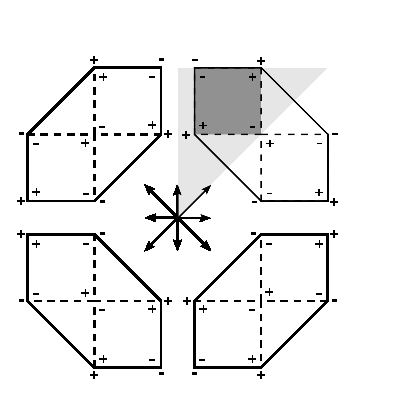
\includegraphics[width=0.95\linewidth]{drawing-1}
\caption{Splint $D_3= B_2\cup A_1+A_1$: the projection of the singular element $\Phi_{D_3}^{[1,1,2]}$ can be made from singular elements $\Phi_{A_1+A_1}^{[1,1]}$. Light-grey area is the fundamental Weyl chamber of subalgebra $B_2$.} 
\label{ris1} 
\end{minipage}
\hfill
\begin{minipage}[h]{0.47\linewidth}
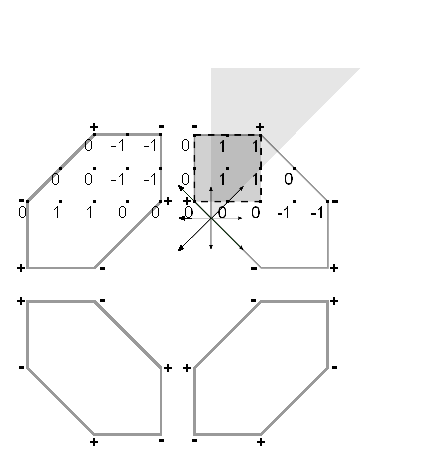
\includegraphics[width=0.9\linewidth,viewport=0 0 157 157,clip]{drawing-3}
\caption{The injection fan applied to the singular element $\Phi_{A_1+A_1}^{[1,1]}$ yields branching coefficients that are equal to 1.}
\label{ris2}
\end{minipage}
\end{center}
\end{figure}

A careful examination of the embedding $G_{2}\to B_{3}$ leads to exactly the same conclusion. 

So far we only considered special splints where both embedded systems are root systems. However, it
is possible to study the splints where it is not the case. Such splints obviously can not serve to
simplify calculation of the branching rules but one may use the properties of special embeddings and
the projections to creat a repesentation theory for the systems that are not root systems.

As the result we see that branching coefficients coincide with weight multiplicities for the splints
in the following table:
\begin{equation}
\label{tab:2}
\begin{array}{cc||c|c}
\hbox{type} & \hspace{0.25in}\Delta \hspace{0.25in} & \hspace{0.25in}\Delta
_{\frak{a}}\hspace{0.25in} & \hspace{0.25in}\Delta _{\sfr}\hspace{0.25in}
\\ \hline\hline
\hbox{(i)} & G_{2} & A_{2} & A_{2} \\
& F_{4} & D_{4} & D_{4} \\ 
\hbox{(*)} & B_{3} & G_{2} & A_{2}  \\
\hbox{(*)} & D_{r+1} & B_{r} & \oplus ^{r}A_{1}  \\
\hline
\hbox{(ii)} & B_{r}(r\geq 2) & D_{r} & \oplus ^{r}A_{1} \\
\hbox{(iii)} & A_{r}(r\geq 2) & A_{r-1}\oplus u\left( 1\right)  & \oplus
^{r}A_{1} \\
& B_{2} & A_{1}\oplus u\left( 1\right)  & A_{2}
\end{array}
\end{equation} 
here the splints marked with (*) are special splints.


\section{Conclusion}
\label{sec:conclusion}

The computation of branching coefficients is important for different physical models with a symmetry
breaking. This computation is drastically simplified if branching coefficients coincide with weight
multiplicities, since efficient Freudental formula can be used \cite{moody1982fast}. The classification
of splints for regular and special embeddings gives us all the cases when this coincidence takes
place. Aside from computational importance, this coincidence is very interesting from
representation-theoretic point of view, because it follows from the new unexpected connection between
different simple Lie algebras. 

There exist special embeddings of semisimple Lie algebras into simple Lie algebras. For such
embeddings the procedure of finding splints that allow to calculate branching coefficient is similar
to the one conducted above. While the results of the procedure are not presented in this paper they
can be obtained with little difficulty.

\section*{Acknowledgements}
\label{sec:acknowledgements}

We thank the organizers of the conference ``In Search of Fundamental Symmetries'' where some results
of this work were presented.

P.I. Kakin would like to acknowledge Saint Petersburg State University for the research grant
11.38.185.2014.


\bibliography{special-bibliography}{} 
\bibliographystyle{utphys}

\end{document}
